\subsection{\forlnameref Aplicación}
\label{sec:applicationTests}

\begin{shaded}
En este ejemplo se presenta únicamente la clase de prueba de \code{User} como representante de otras clases de la lógica.
\end{shaded}

\lstinputlistingContent{language=java,caption={Java - Clase \code{UserTest} de pruebas unitarias para clase \code{User}}}{tests/unitTests/UserTest.java}

La Figura \ref{fig:eclipseJUnit} (pág. \pageref{fig:eclipseJUnit}) muestra el resultado de la ejecución del conjunto de pruebas unitarias del archivo \code{UserTest.java}.

\begin{landscape}
\setcaptiontype{figure}
\centering
\frame{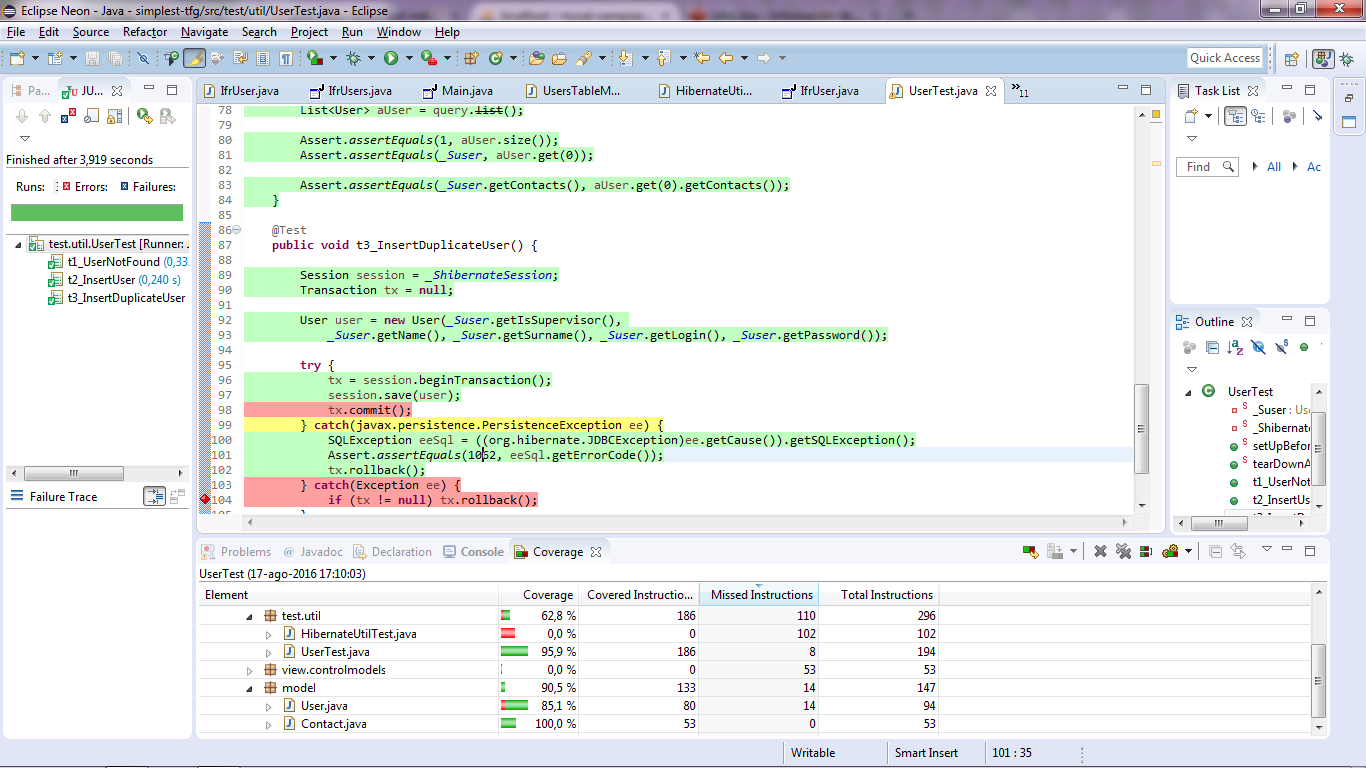
\includegraphics[scale=0.62]{eclipseJUnit.png}}
\caption{Ejemplo de pruebas unitarias con cobertura de código sobre la clase \code{User}}
\label{fig:eclipseJUnit}
\end{landscape}